The first part of our fitting algorithm is to fit the protein backbone to the given \Ca-trace ignoring the side-chain conformations.

As input we are given a \Ca-trace target and a protein in form of an amino acid sequence.
Only the amino acid types are provided; no spatial structure information about the protein is given as this is left to the fitting algorithm to find.


\section{Limitations}
The adjustable parameters in a protein backbone structure consists of bond angles, dihedral angles and bond lengths.
As the dihedral angles are by far the most influential parameters w.r.t the overall protein structure, we allow ourselves to perform the simplification of not considering bond lengths and bond angles.
More specifically, we will only consider the $\phi$ and $\psi$ angles and use known constants backbone structure template for all other parameters.
Thus, the protein backbone to be folded becomes a sequence of identical amino acid backbones that can only be modified by adjusting $\phi$ and $\psi$ for each amino acid.


\section{Inverse kinematics}
With the above limitations in place the backbone fitting problem can be regarded as an inverse kinematics (IK) problem.
IK is the process of determining angles of joints in a chain of rigid links in order to achieve a desired pose of the entire spatial structure.
In our case, the spatial structure consists of a series of atom bonds (links) connected by atoms (joints).
The desired pose is the \Ca-target.
%simply to make a \Ca-atom in the protein come as close as possible to its corresponding \Ca-trace target.
\fxfatal{skal vi indsætte en simpel IK-illustration her?} 
As we have decided not to consider the bond angles (joint angles), the only adjustable angles in the kinematic chain are the dihedral angles around the atom bonds.

Several IK methods exist and have been utilized in protein structure prediction:
\cite{shenkin1987} describe a Jacobian solution that provide a linear approximation capable of handling lower limit constraints on interatomic distances between certain atoms.
The partial derivatives in the Jacobian matrix models the movement of the end of the kinematic chain relative to the angular changes.
To calculate the necessary changes in the available angles, the Jacobian is inverted.
According to \cite{canutescu2003} this inversion may be ill posed if the Jacobian is close to singular.


%inverse kinematics methods calculate the necessary changes in the available angles to minimize the distance between an object (called the \emph{end effector}) and a desired destination.



%We begin from one end of the amino acid sequence by placing the first two amino acids such that they match the beginning of the \Ca-trace target.


%$||N - C|| \rotateAround{180^\circ} \rotateAround{90^\circ} \rotateAround{v}$

\begin{figure}
  \centering
	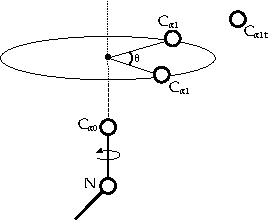
\includegraphics[width=0.75\columnwidth]{figures/ccd_angles}
	\label{fig:ccd_angles}
  \caption{}
\end{figure}

